\documentclass[titlepage]{article}
\usepackage{graphicx}

\title{CS440 - Artificial Intelligence \\ Assignment 1 (3 Credit Hours)}
\author{Jon Reynolds (jdrynld2) \\ Matthew Krikorian (krikorn2) \\ Patrick McMahon (pfmcmah2)}

\begin{document}
\maketitle

\section{Abstract}
In this assignment we explore the different search algorithms that can be used to traverse a maze, and analyze the optimality's and general performance between the different implementations under a very heavy scope. In section 1.1 (basic pathfinding), we analyzed four different pathfinding algorithms. Specifically, Depth-first search, Breadth-first search, Greedy best-first search, and A* search. In section 1.2 (search with multiple dots), we were tasked with developing our own heuristic in the implementation of our A* search algorithm. There are also multiple goal positions in section 1.2 as well, which is why coming up with an admissible heuristic to optimally traverse the mazes was paramount.

\section{Basic Pathfinding} 
In this part of the assignment we implemented four different search algorithms to analyze cost, number of nodes expanded, and overall solution optimality. We were given three different mazes to run our search algorithms on, demonstrating to us the potential pros and cons of each algorithm. \textbf{Breadth-first search} is a search algorithm where the root node is expanded first, then all of the root-notes children are expanded, and so forth until the goal successor (or state) is found. 

\begin{figure}[h!]
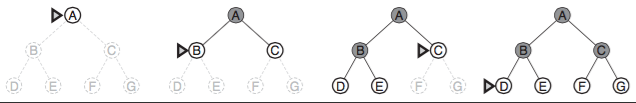
\includegraphics[width=\linewidth]{bfs.png}
\caption{Breadth-first search algorithm, \textit{Russell and Norvig}}
\label{fig:BFSdiagram1}
\end{figure}

\noindent
\textbf{Depth-first search} is a search algorithm where the deepest node currently in the frontier is always chosen to be expanded with the hope of finding the goal state. If the goal state is not found once the algorithm finds a node with no successors, the algorithm will then backtrack back to the next deepest node that still has unexplored successors.

\newpage

\begin{figure}[h!]
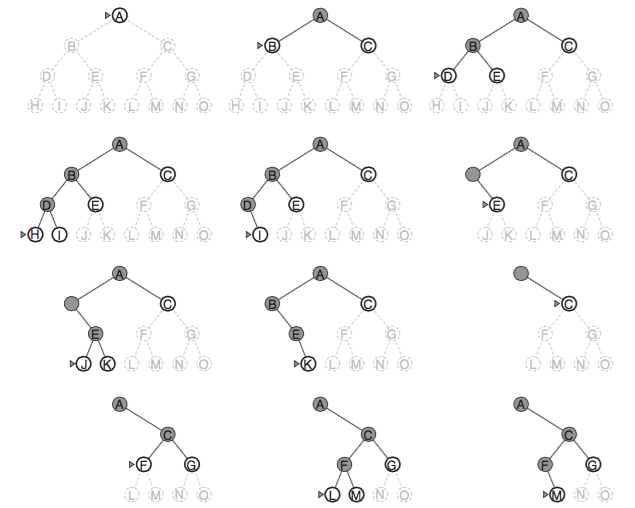
\includegraphics[width=\linewidth]{dfs.png}
\caption{Depth-first search algorithm, \textit{Russell and Norvig}}
\label{fig:DFSdiagram1}
\end{figure}

\noindent
\textbf{Greedy best-first search} is a search algorithm that always chooses to go down the path that has the lowest cost with respect to the other neighbors of the current node it is on. The name greedy implies that it does not care about the actions of the future, but rather only chooses it's path on the best choice to it based on immediate cost. Greedy algorithms evaluate the nodes they are going to travel to using a heuristic function. This heuristic does not use past or future information to make any decisions, which sets it apart from both the BFS and DFS search algorithms. The algorithm chooses the next node it will travel to directly from the heuristic function it is given, so the choosing function \(f(n)\) can be modeled as \(f(n) = h(n)\) where \(h(n)\) is the heuristic function.\newline
\newline
Finally, \textbf{A* search} is a search algorithm where the function used to evaluate which node the algorithm will travel to next, \(f(n)\), is dependent on both the cost from the start node to the goal node, \(g(n)\), and the cost to get from the current node to the goal node, \(h(n)\). The node selection function is actually modeled as the direct sum of \(h(n)\) and \(g(n)\), giving us \(f(n) = h(n) + g(n)\). This algorithm is thought of as the algorithm amongst the four that often provides the most savings, and can be optimized heavily through a very good heuristic function \(h(n)\).

\subsection{Our Code, Explained}
Start talking about our code here



\end{document}


























